\documentclass[12pt]{article}

\usepackage{sbc-template}

\usepackage{graphicx,url}

\usepackage[utf8]{inputenc}  
\usepackage[brazil]{babel}  

\graphicspath{ {./img/ptbr} }

\makeatletter
\def\input@path{{./sections/ptbr}}
\makeatother
     
\sloppy

\title{Estudo Comparativo de Mecanismos de Segurança Aplicados à Autenticação e Autorização em 
Sistemas Web}

\author{Rafael Strack\inst{1}, Adriano Ferrasa\inst{1}}

\address{Departamento de Informática -- Universidade Estadual de Ponta Grossa
  (UEPG)\\
  84.030-900 -- Ponta Grossa -- PR -- Brasil
\email{rafa\_strack@hotmail.com, ferrasa@uepg.br}
}
\begin{document}

\maketitle

\begin{abstract}
  This article presents a comparative study of authentication and authorization mechanisms in web
  systems, aiming to provide an in-depth analysis of the available options and their
  characteristics. The study describes the most commonly used methods in the field, such as passwords, 
  tokens, OAuth and OpenID Connect, analyzing their advantages and disadvantages, as well as the usage 
  flow of each method. In the end, a comparison of the studied methods is conducted, evaluating their 
  effectiveness in terms of security. A proper understanding of these mechanisms is essential to ensure 
  the security of web systems and to guide the correct choice in future projects.
\end{abstract}

\begin{resumo}
  Este artigo apresenta um estudo comparativo de mecanismos de autenticação e autorização em
  sistemas web, visando fornecer uma análise aprofundada das opções disponíveis e suas
  características. O estudo descreve os métodos mais utilizados na área, como senhas, tokens, OAuth 
  e OpenID Connect, analisando suas vantagens e desvantagens, bem como o fluxo de utilização de 
  cada método. Ao final, é realizada uma comparação dos métodos estudados, avaliando-se sua eficácia 
  em termos de segurança. A compreensão adequada desses mecanismos é fundamental para garantir a 
  segurança dos sistemas web e orientar a escolha correta em projetos futuros.
\end{resumo}

\section{Introdução}

Com a expansão da internet, os sistemas web assumiram um papel crucial no cotidiano de bilhões de
pessoas em todo o mundo. Desde o uso de aparelhos domésticos até o gerenciamento de 
negócios online, esses sistemas se tornaram indispensáveis para diversas atividades 
\cite{GREENGARD2015}. No entanto, a segurança desses sistemas é uma preocupação constante para 
desenvolvedores e usuários, pois há uma série de ameaças e vulnerabilidades que podem comprometer 
sua integridade.

A fundação OWASP (\emph{Open Worldwide Application Security Project}) atualiza regularmente um
relatório chamado OWASP Top 10, onde são descritos os 10 riscos de segurança mais críticos em
sistemas web. Na última edição, realizada em 2021, a categoria que ficou em primeira colocação foi
a quebra de controle de acesso. Em sétima colocação, ficou a categoria de falhas de identificação e
autenticação \cite{OWASP2021}. Esses problemas são diretamente relacionados aos processos de
autenticação e autorização de usuários, os quais são essenciais para garantir a proteção adequada
dos sistemas.

De modo geral, a autenticação é o processo de validação de usuários, enquanto a autorização é o
método que fornece as permissões de acesso corretas aos recursos para usuários previamente
autenticados \cite{TUMIN2012}. Atualmente, existem diversos mecanismos de autenticação e autorização
de usuários disponíveis, como senhas, \emph{tokens}, autenticação multifator, OAuth, OpenID, entre
outros. Cada um desses mecanismos apresenta características distintas, pontos positivos e negativos,
sendo fundamental garantir a correta implementação dos mecanismos escolhidos, de forma a assegurar
a efetividade da segurança dos sistemas web.

Diante desse contexto, o presente trabalho tem como objetivo realizar um estudo
comparativo dos diferentes mecanismos de autenticação e autorização, com o propósito
de fornecer uma análise aprofundada que auxilie na escolha adequada desses mecanismos
em projetos de sistemas web. O estudo visa oferecer uma compreensão ampla das
características, pontos fortes e limitações de cada mecanismo, permitindo a seleção
correta e a implementação eficiente das medidas de segurança necessárias.

\section{Autenticação e Autorização}

Na maioria dos sistemas \emph{web}, é necessário realizar um controle de acesso para que somente
certos usuários possam acessar recursos protegidos. Para isso, o mecanismo  de controle de
acesso depende de dois processos relacionados: a autenticação e a autorização
\cite{SULLIVAN2011}.

A autenticação pode ser definida como o processo de confirmação de identidade. Porém, em sistemas 
\emph{web}, devido a falta de conhecimento do mundo real, este processo pode não ser simples
\cite{CHAPMAN2012}. Existem três grupos de fatores amplamente utilizados para confirmar a
identidade de um usuário: algo que o usuário sabe, algo que o usuário é e algo que o usuário
possui. No primeiro grupo, inclui-se as senhas, PINs (\emph{Personal Identification Number}) e
frases secretas. No segundo grupo, inclui-se certificados digitais, \emph{smart cards} e
\emph{tokens} de segurança. O terceiro grupo inclui técnicas biométricas, como como impressões
digitais, reconhecimento facial ou de voz, entre outras \cite{SULLIVAN2011}.

De forma complementar, a autorização é o processo pelo qual o sistema verifica se um usuário 
previamente autenticado possui permissão para acessar um recurso ou executar uma determinada ação 
\cite{SPILCA2020}. Ela pode ser realizada de várias formas, porém as mais comuns são as baseadas em 
usuários, perfis (\emph{roles}) e com o uso do protocolo OAuth \cite{CHAPMAN2012}.

\subsection{Autenticação Básica HTTP}

A autenticação básica HTTP (\emph{Hypertext Transfer Protocol}) foi definida na especificação
HTTP/1.0 \cite{RFC1945}, porém tornou-se um padrão na RFC 2617 \cite{RFC2617}. Neste tipo de
autenticação, o servidor web recusa uma transação caso o cliente não esteja autenticado,
desafiando-o para obter um nome de usuário e senha válidos. Este desafio de autenticação é iniciado
retornando o status HTTP 401 (não autorizado) e especificando o domínio de segurança
(\emph{security realm}) a ser acessado, com o cabeçalho \texttt{WWW-Authenticate}. Ao receber o 
desafio, o cliente abre uma caixa de diálogo para que o usuário insira as credenciais para acesso 
ao domínio. O cliente então junta as informações de usuário e senha, colocando dois pontos entre 
eles, e os codifica usando o método de codificação base-64. Estas credenciais codificadas são 
colocadas no cabeçalho \texttt{Authorization}, e então a requisição é enviada para o servidor, que 
fará a validação das credenciais e, caso validadas, retorna-se o status HTTP 200 (OK) 
\cite{GOURLEY2002} (Figura \ref{fig:basicAuth}).

\begin{figure}[ht]
  \centering
  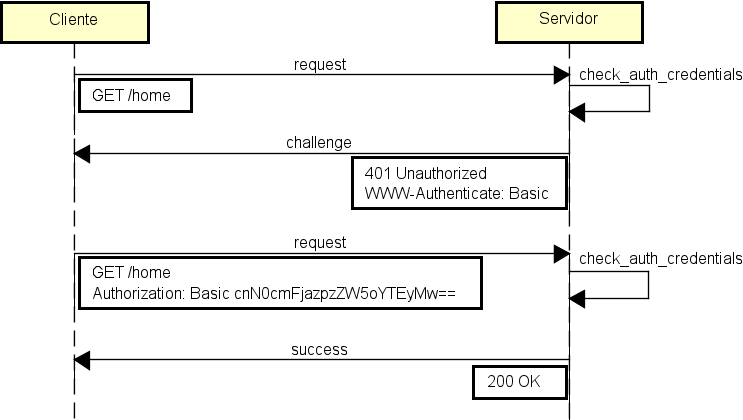
\includegraphics[width=.8\textwidth]{Basic Authentication.png}
  \caption{Exemplo de autenticação básica HTTP}
  \label{fig:basicAuth}
\end{figure}

A diretiva de domínio (\emph{realm}) utilizada nas autenticações HTTP define os espaços de proteção 
do sistema web. Esses domínios permitem que os recursos protegidos sejam particionados, cada um com 
seu próprio esquema de autenticação e/ou autorização \cite{RFC2617}.



\subsection{Autenticação \emph{Digest} HTTP}

A autenticação \emph{Digest} foi especificada na RFC 2019 \cite{RFC2019}, porém também foi 
realocada para a RFC 2617. Foi desenvolvida para ser uma alternativa mais compatível e segura  para 
a autenticação básica, corrigindo as falhas mais graves da mesma, como a falta de criptografia de 
senhas, vulnerabilidade a captura e reprodução de pacotes e proteção contra vários outros tipos 
comuns de ataques \cite{GOURLEY2002}.

Assim como a autenticação básica HTTP, a \emph{Digest} é baseada no paradigma 
desafio-resposta \cite{RFC7616}. A diferença é que foram adicionados diversos parâmetros nos 
cabeçalhos, para identificação única de desafios, nível de qualidade de proteção, especificação de 
algoritmo de hashing utilizado entre outros recursos \cite{CHAPMAN2012}. Por padrão, o algoritmo 
utilizado é o MD5, porém na RFC 7616 foram adicionados e recomendados os algoritmos SHA-256 e 
SHA-512/256 \cite{RFC7616}.

O parâmetro \texttt{response} é a principal parte do cabeçalho \texttt{Authorization}: ele contém 
uma concatenação criptografada de dados da requisição, como nome do usuário, \texttt{realm}, senha, 
método HTTP, URL, entre outros parâmetros, todos separados por dois pontos. \cite{CHAPMAN2012}. O 
cliente realiza o cálculo resultante no valor de \texttt{response}. O servidor também o faz e 
compara com o valor recebido. Caso as credenciais sejam válidas, retorna-se o status HTTP 200 (OK)
e o cabeçalho \texttt{Authentication-Info}, que contém parâmetros utilizados para uma futura 
autenticação, autenticação mútua e reenvio de parâmetros para confirmação de legitimidade. Um 
exemplo do funcionamento deste método de autenticação é mostrado na Figura \ref{fig:digestAuth}.

\begin{figure}[ht]
  \centering
  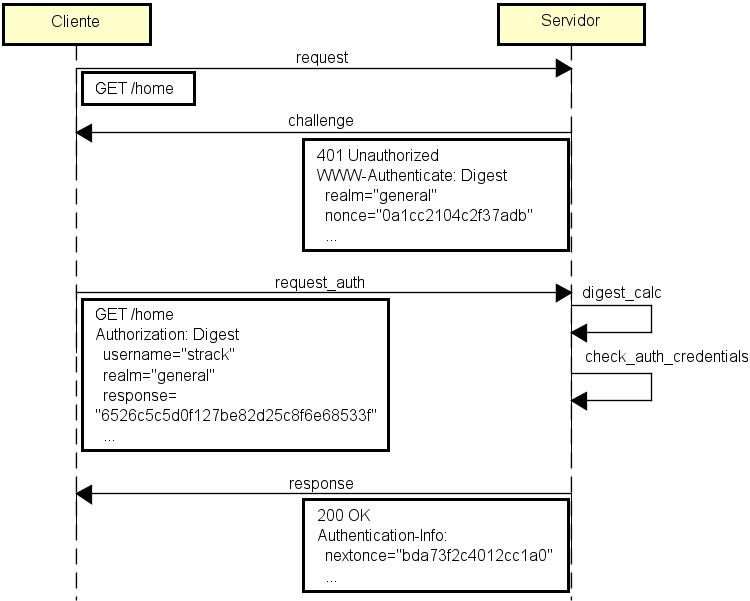
\includegraphics[width=.8\textwidth]{Digest Authentication (Simplified).png}
  \caption{Exemplo de autenticação \emph{Digest}}
  \label{fig:digestAuth}
\end{figure}

\subsection{Autenticação Baseada em Sessão}

Uma sessão web é uma troca de informações semipermanente entre um cliente e um servidor web 
\cite{CALZAVARA2017}. O mecanismo de gerenciamento de estados para o HTTP, baseado em sessões, foi 
especificado na RFC 2109 \cite{RFC2109} com sua versão mais atual especificada na RFC 6265 
\cite{RFC6265}. Este mecanismo utiliza o termo \emph{cookie} para se referir às informações de 
estados que são passadas entre o servidor e o cliente, e salvas no cliente \cite{RFC2109}. 

A autenticação baseada em sessão é o método mais comum de autenticação em sistemas web. Neste 
método, após o envio de credenciais de acesso e validação do usuário por meio de uma requisição 
HTTP, o servidor gera um \emph{cookie}, armazena-o e envia-o pelo cabeçalho \texttt{Set-Cookie} da 
resposta para o cliente. O cliente salva o valor, que é enviado no cabeçalho \texttt{Cookie} em 
toda requisição para o mesmo servidor de origem \cite{PAPATHANASAKI2022} (Figura \ref{fig:sessionAuth}).

\begin{figure}[ht]
  \centering
  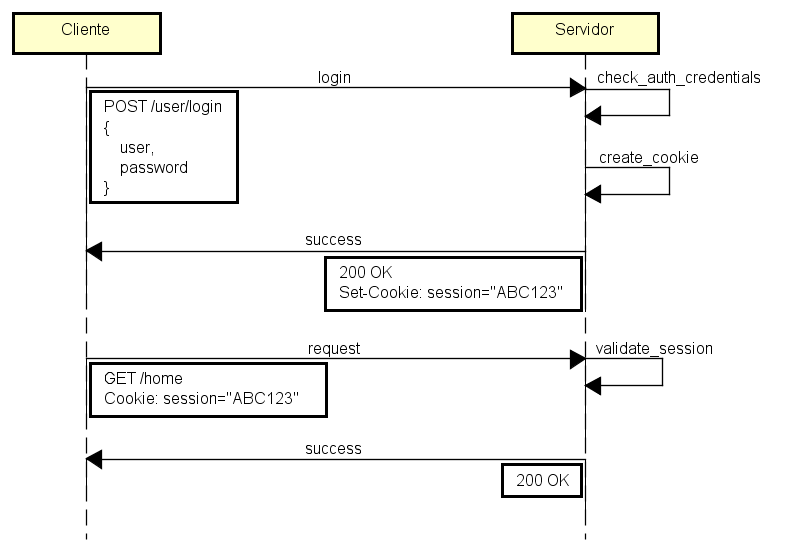
\includegraphics[width=.8\textwidth]{Session-Based Authentication.png}
  \caption{Exemplo de Autenticação baseada em sessão}
  \label{fig:sessionAuth}
\end{figure}

\subsection{Autenticação Baseada em Token}

\emph{Tokens} são itens utilizados para identificar e autenticar usuários. São palavras assinadas e 
não criptografadas, que carregam informações sobre um usuário autenticado \cite{BALAJ2017}. O 
padrão mais utilizado deste tipo de autenticação é o JSON \emph{Web Token} (JWT), que foi proposto
na RFC 7519. O JWT é um formato compacto de representação de reinvindicações (\emph{claims}), 
destinado a ambientes com restrição de espaço, como cabeçalhos HTTP e parâmetros de consulta de URI 
(\emph{Uniform Resource Identifier}) \cite{RFC7519}.

Um JSON \emph{Web Token} é composto por cadeias de caracteres codificadas em \emph{base64url} (codificação
\emph{base64} com alterações para uso em URLs e nomes de arquivo), separadas 
por ponto. Geralmente possuem 3 cadeias: o cabeçalho, que contém informações a respeito do tipo de mídia do 
JWT e da criptografia usada para assinar o \emph{token}; a carga útil (\emph{payload}), que contém 
as informações sobre as \emph{claims}, que são conjuntos de declarações sobre uma entidade 
(geralmente um usuário); e a assinatura, que é a concatenação dos \emph{hashes} gerados a partir das 
outras duas cadeias com uma chave secreta ou certificado, utilizada para verificação de integridade
do \emph{token} \cite{MONTANHEIRO2017}.

Neste método, após o envio de credenciais de acesso e validação do usuário por meio de uma 
requisição HTTP, o servidor gera um \emph{token}, que é enviado para o cliente e pode ser salvo
em \emph{cookies} ou no armazenamento local \cite{MONTANHEIRO2017}. Também pode ser enviado um 
\emph{token} de atualização (\emph{refresh token}), para a obtenção de um novo \emph{token} de acesso
assim que o atual expirar. Ao possuir o \emph{token}, quando uma requisição é feita ao servidor o 
mesmo deve ser enviado no cabeçalho \texttt{Authorization}, precedido pela palavra \emph{Bearer}. 
\cite{RFC6749} (Figura \ref{fig:tokenAuth}).

\begin{figure}[ht]
  \centering
  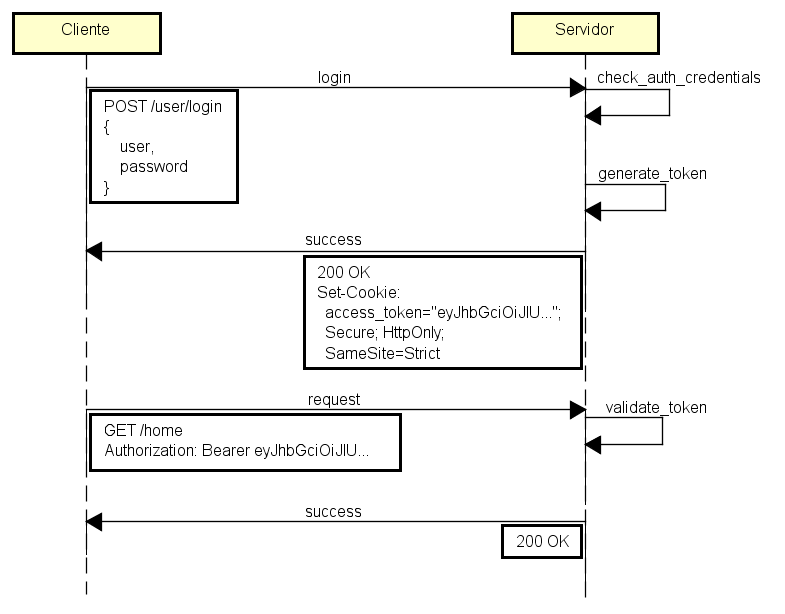
\includegraphics[width=.85\textwidth]{Token-Based Authentication.png}
  \caption{Exemplo de Autenticação baseada em \emph{token}.}
  \label{fig:tokenAuth}
\end{figure}

\

\

\subsection{OAuth e OAuth 2.0}

O protocolo OAuth foi especificado na RFC 5849, fornecendo um método para clientes acessarem 
recursos de um servidor em nome de um proprietário de recurso e também um processo para que os 
usuários finais autorizem o acesso de terceiros aos seus recursos de servidor sem compartilhar suas
credenciais \cite{RFC5849}. Este método de autenticação funciona seguindo as seguintes etapas:

\begin{itemize}
\item O usuário solicita o serviço de um sistema, chamado de cliente;
\item O cliente, tendo previamente configurado acesso ao servidor de recursos, possuindo um 
identificador e um segredo compartilhado, envia uma solicitação a este servidor para receber um 
\emph{token} de solicitação;
\item O servidor valida a solicitação, enviando o \emph{token} de solicitação não-autorizado no 
corpo da resposta HTTP;
\item O cliente redireciona o agente do usuário para o servidor, que solicita o \emph{login} do 
usuário e depois a autorização para o cliente acessar o recurso;
\item O cliente recebe um \emph{token} de solicitação, que utiliza em uma nova solicitação por 
\emph{token} de acesso. Estas requisições são realizadas por meio de um canal TLS;
\item O servidor valida o \emph{token} de solicitação e envia o \emph{token} de acesso ao cliente e 
opcionalmente um \emph{token} de atualização;
\item O cliente utiliza o \emph{token} de acesso para solicitar os recursos do servidor.
\end{itemize}

Na RFC 6749 foi proposto o protocolo OAuth 2.0, tornando obsoleta sua versão anterior. Esta versão possui 
poucas semelhanças com a versão anterior, utilizando os mesmos princípios mas com fluxo diferente e 
abrangendo mais casos de uso, além de estabelecer o uso do protocolo HTTPS, possuindo todas as mensagens 
criptografadas. Por este motivo os dois protocolos não são compatíveis, coexistindo e podendo ambos serem 
suportados pelos sistemas \cite{RFC6749}. Diferente da versão 1.0, que depende de assinaturas 
criptografadas para cada requisição, a versão 2.0 utiliza \emph{tokens} portadores (\emph{bearer tokens}) 
que são protegidos devido ao uso do TLS \cite{SIRIWARDENA2014}. Seu funcionamento é dado pelas seguintes 
etapas (Figura \ref{fig:OAuth2}):

\begin{itemize}
\item O cliente solicita permissão de acesso ao usuário;
\item O cliente recebe a permissão e solicita um \emph{token} de acesso ao servidor de autenticação;
\item O servidor de autenticação autentica o cliente e valida suas permissões, enviando a ele o 
\emph{token} de acesso e opcionalmente um \emph{token} de atualização;
\item O cliente solicita o recurso protegido ao servidor de recursos, que valida o \emph{token} de 
acesso e atende a solicitação.
\end{itemize}

\begin{figure}[ht]
    \centering
    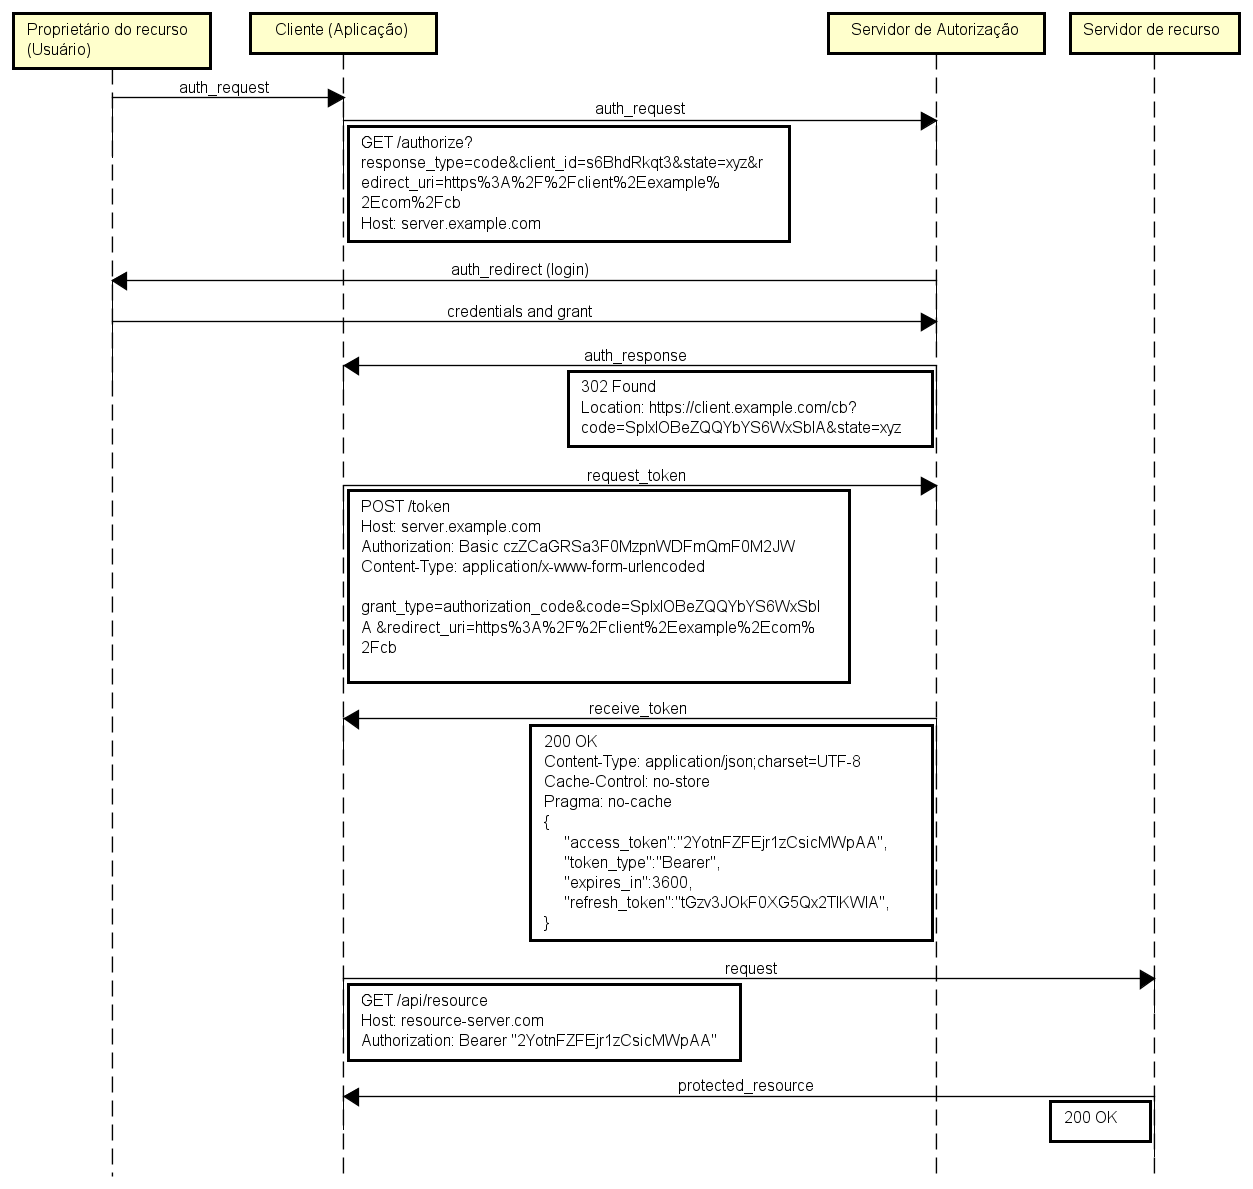
\includegraphics[width=1\textwidth]{OAuth 2.0.png}
    \caption{Exemplo de autenticação utilizando OAuth 2.0}
    \label{fig:OAuth2}
\end{figure}

\subsection{OpenID Connect}

O OpenID Connect (OIDC) é um padrão de camada de identificação em cima do protocolo OAuth 2.0. Utiliza 
todos os conceitos, \emph{tokens} e fluxos do protocolo OAuth 2.0, com a adição do fornecimento de 
atributos do usuário. Esses atributos podem ser 
fornecidos para um sistema por meio de uma API RESTful \texttt{userinfo} ou por meio de um 
\emph{token} de identificação \cite{BIEHL2019}.

O OIDC implementa autenticação como uma extensão da autorização fornecida pelo protocolo OAuth 2.0 
\cite{OIDCCORE}. Similar com o fluxo do OAuth, este método segue as seguintes etapas:

\begin{itemize}
    \item O cliente redireciona para o servidor de autenticação (Provedor OIDC) com os parâmetros 
    necessários (ID do cliente, URI de redirecionamento, etc.);
    \item O provedor apresenta uma página de login ao usuário;
    \item Após login bem sucedido, é solicitada a permissão de acesso aos recursos para o usuário;
    \item O provedor OIDC redireciona o usuário ao cliente, com o código de autorização;
    \item O cliente solicita ao provedor OIDC um \emph{token} de identificação e também geralmente
\emph{tokens} de acesso e atualização;
    \item O provedor envia ao cliente os \emph{tokens} que podem ser utilizados para acessar 
informações do usuário (\emph{endpoint} \texttt{userinfo}), recursos protegidos e solicitar novos 
\emph{tokens} \cite{OIDCCORE}.
\end{itemize}

Um exemplo de funcionamento de uma autenticação utilizando OIDC é mostrado na figura 
\ref{fig:OpenID}

\begin{figure}[ht]
    \centering
    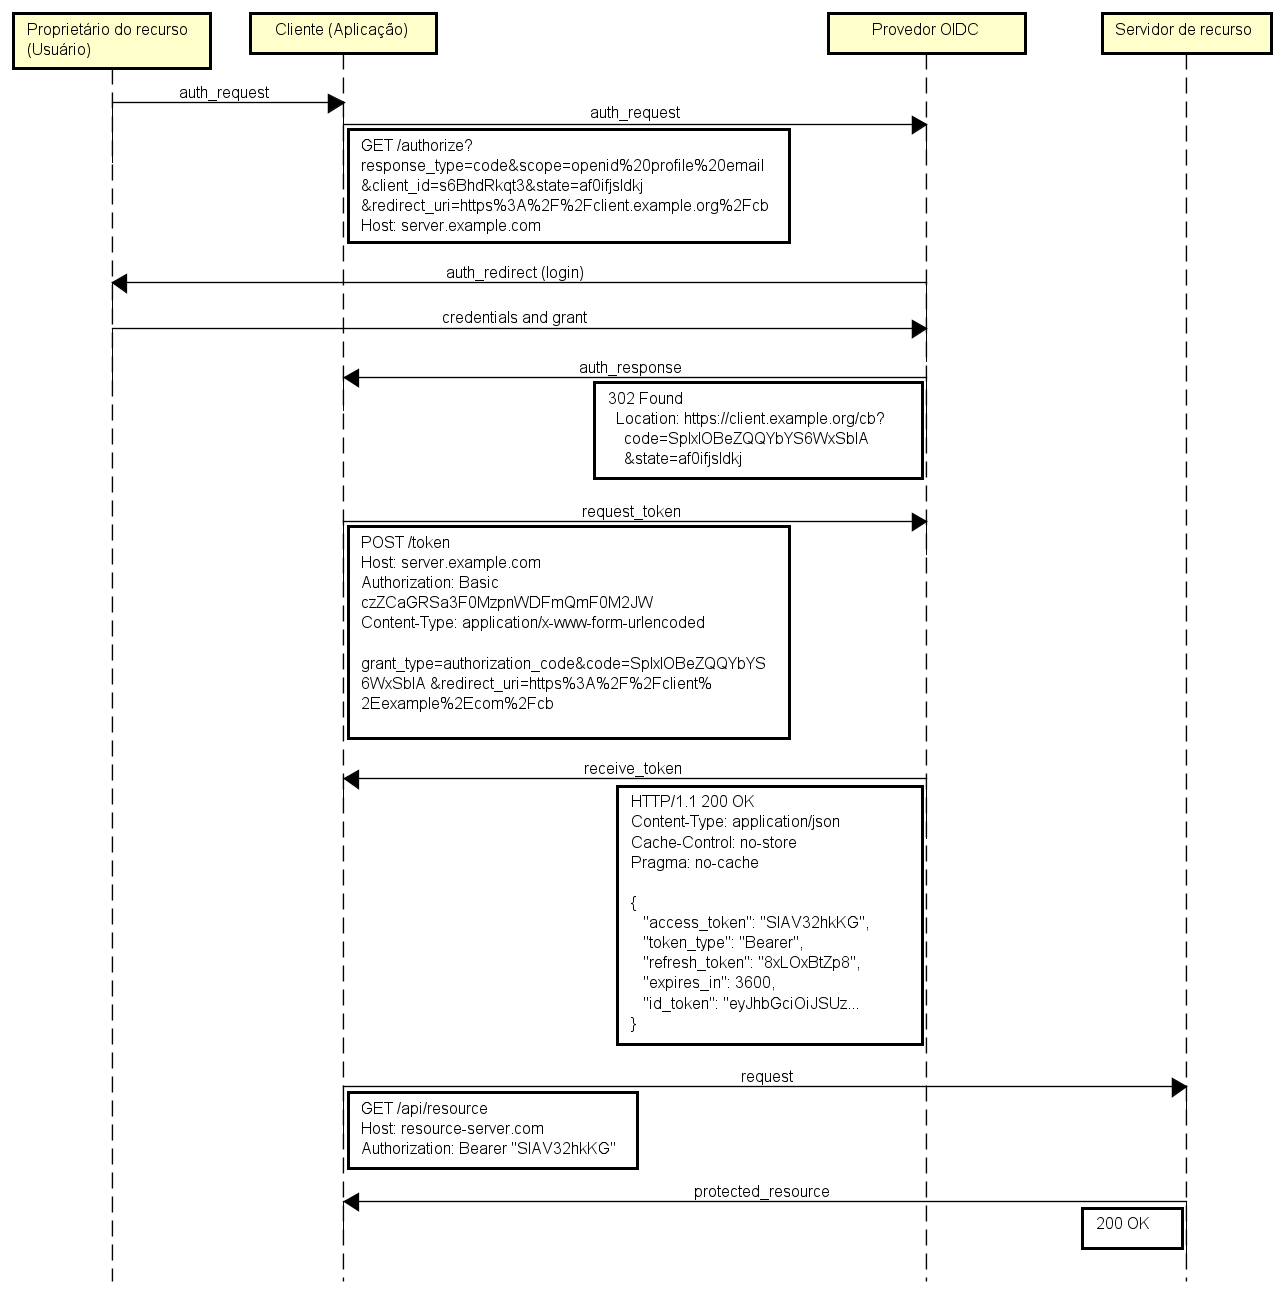
\includegraphics[width=0.95\textwidth]{OpenID Connect.png}
    \caption{Exemplo de autenticação utilizando OpenID Connect}
    \label{fig:OpenID}
\end{figure}

\section{Materiais e Métodos}



\section{Resultados e Discussão}

%%%%% Basic
A autenticação básica HTTP é simples e de fácil implementação, porém não possui mecanismos de 
garantia efetiva de segurança. As credenciais do usuário podem ser facilmente decodificadas, visto 
que a codificação base64 é facilmente reversível, podendo ser realizada em poucos segundos. Também 
é possível realizar ataques de repetição, visto que terceiros podem capturar pacotes e replicá-los, 
mesmo que codificados, podendo obter acesso ao sistema. Este tipo de autenticação não possui proteção 
contra \emph{proxies} ou \emph{middlewares}, que podem facilmente modificar o corpo da mensagem, e 
também são vulneráveis a servidores falsificados, que se passam por outros para realizar o roubo de 
credenciais \cite{GOURLEY2002}.

Além destes pontos negativos, a autenticação básica não possui desconexão, pois o navegador mantém 
os dados em \emph{cache} por padrão, até ser fechado. A documentação deste método cita a sua falta 
de segurança, indicando seu uso somente para propósitos simples de identificação, sem risco de 
acesso a informações sensíveis ou valiosas \cite{RFC7617}. 

%%%%% Digest
Apesar da grande melhora de segurança em relação a autenticação básica, a autenticação 
\emph{Digest} ainda possui diversos riscos de segurança. Os cabeçalhos 
\texttt{WWW-Authenticate} e \texttt{Authorization} possuem certo nível de proteção a manipulação, 
porém todos os outros cabeçalhos não possuem. Ataques de repetição podem ser realizados se a 
implementação de identificadores únicos por desafio não for realizada. Caso não seja estabelecida 
nenhuma política de força de senha, podem ser realizados ataques de dicionário, tentando adivinhar 
a senha e outros parâmetros, visto que o nome do usuário é obtido sem esforço. Se a requisição 
passar por \emph{proxies} hostis ou comprometidos, o cliente pode ficar vulnerável a ataques 
\emph{man-in-the-middle} \cite{GOURLEY2002}. 

Assim como a autenticação básica, a Digest não possui desconexão, possuindo o mesmo problema citado
anteriormente. Sua documentação cita que, pelos padrões modernos de criptografia, este método 
é fraco, porém um substituto muito superior a autenticação básica \cite{RFC7616}.

%%%%% Session
Em relação à autenticação baseada em sessão, a grande vantagem é a diminuição do envio das 
credenciais do usuário nas requisições, diminuindo a janela de ataques, já que os \emph{cookies} 
são utilizados para a validação das requisições. Por outro lado, os cookies podem ser lidos por 
outros aplicativos, tornando o sistema exposto a ataques \emph{Cross Site Scripting} (XSS) e 
\emph{Cross Site Request Forgery} (CSRF). Para evitar ataques XSS, pode-se definir no \emph{cookie} 
a \emph{flag} \texttt{http-only}, que faz com que o acesso por APIs do lado cliente seja negado 
\cite{PAPATHANASAKI2022}. 

Existe a possibilidade do ataque de fixação de sessão, onde o atacante insere seu próprio valor
dentro do \emph{cookie}, esperando o usuário entrar no sistema com esse identificador. Se o servidor
aceitá-lo, o atacante obtém acesso ao servidor, podendo obter informações privadas sobre a vítima
e realizar ações usando sua identidade \cite{DRHOVA2018}.

Se não forem transportados por um canal seguro, como TLS, as informações nos cabeçalhos referentes 
aos \emph{cookies} podem ser visualizadas. Por este motivo, além de enviados por um canal seguro, 
os \emph{cookies} devem ser criptografados e assinados pelo servidor\cite{RFC6265}.

A autenticação baseada em sessão é \emph{stateful}, contendo todos os identificadores de sessão do
lado do servidor, causando uma sobrecarga no mesmo e dificultando o gerenciamento dessas sessões em
múltiplos servidores, diferentemente das outras técnicas abordadas, que são \emph{stateless} 
\cite{BALAJ2017}.

%%%%% Token

Sobre a autenticação baseada em \emph{tokens}, mais especificamente utilizando JWT, que é a mais 
comum, pode-se listar algumas vulnerabilidades, caso boas práticas não sejam aplicadas. Caso seja
validado pelo servidor o uso de JWTs sem assinatura, pode-se sofrer ataque de remoção de assinatura,
removendo a terceira parte do \emph{token} e alterando seu cabeçalho. Caso os \emph{tokens} sejam
armazenados em \emph{cookies}, é possível a realização de ataques CSRF, além de ataques XSS, caso a
\emph{flag} \texttt{http-only} não seja declarada \cite{PEYROTT2018}. Caso a chave de assinatura
do JWT possua baixa entropia, um ataque de força-bruta pode ser realizado para descobri-la 
\cite{RFC7515}.

%%%%% OAuth
O protocolo OAuth quando foi publicado, em 2007, tornou-se rapidamente o padrão na indústria para 
delegação de acesso na web. Porém, teve problemas no domínio empresarial, devido ao seu desempenho. 
A comunidade percebeu que o protocolo não era escalável: exige gerenciamento de estado em diferentes 
etapas, gerenciamento de credenciais temporárias e não fornece isolamento do servidor de autorização 
do próprio servidor de recursos protegidos \cite{NOUREDDINE2011}. O OAuth 2.0 resolveu estes 
problemas, facilitando o fluxo ao substituir as assinaturas por \emph{bearer tokens}, utilizando TLS 
durante todo o fluxo, não somente no \emph{handshake} inicial e definindo o servidor de autorização 
separadamente do servidor de recurso, que traz maior flexibilidade \cite{SIRIWARDENA2014}.

Em relação a ataques, ambos são suscetíveis a CSRF. A versão 1.0 é mais suscetível devido a 
falta de uso de TLS em todo seu fluxo, enquanto a versão 2.0 é suscetível a este ataque caso as 
diretrizes de implementação não forem seguidas \cite{FETT2016}. Também acaba se tornando suscetível 
a ataques de \emph{phishing} e \emph{spoofing}, caso não forem seguidas as diretrizes \cite{RFC6819}

%%%%% OIDC

O OpenID Connect, por ser uma camada sobre o protocolo OAuth 2.0, possui muitas vulnerabilidades 
em comum com este. Porém, o OIDC possui algumas em particular que são aplicadas somente a
ele: ataques de falsificação de solicitações no servidor, que são facilitados pela descoberta 
\emph{ad hoc} e pelos recursos de registro dinâmico; ataques de injeção, permitidos devido aos mesmos
recursos; ataques CSRF, devido ao recurso de inicialização de login de terceiros e ataques ao
/emph{token} de identificação, que não existe no OAuth \cite{FETT2017}.

Da mesma forma, algumas das vulnerabilidades do OAuth 2.0 não são aplicadas ao OIDC: 
suas configurações são menos propensas a ataques de redirecionamento aberto, uma vez que 
\emph{placeholders} não são permitidos em URIs de redirecionamento; o TLS é obrigatório para 
algumas mensagens no OIDC, enquanto é opcional no OAuth 2.0; o valor \texttt{nonce} pode evitar 
alguns ataques de repetição quando o valor do estado não é usado ou vaza para um invasor 
\cite{FETT2017}.

\begin{table}[ht]
\centering
\caption{Tabela comparativa entre aspectos de ferramentas de autenticação e autorização}
\label{tab:comparativeTable}
\begin{tabular}{|l|l|l|l|l|}
% Cabeçalho
\hline
Mecanismo
% & Usabilidade
& \begin{tabular}[c]{@{}l@{}}Nível de \\ Segurança\end{tabular}
& Vulnerabilidades
% & \begin{tabular}[c]{@{}l@{}}Facilidade de \\ Implementação\end{tabular}
& Obsolescência
\\ \hline

% Basic Auth
\begin{tabular}[c]{@{}l@{}}HTTP Basic \\ Authentication\end{tabular}
% & Baixa
& \begin{tabular}[c]{@{}l@{}}Extremamente \\ baixo\end{tabular}   
& \begin{tabular}[c]{@{}l@{}}Força-Bruta\\Interceptação\\Reprodução\\\emph{Man-in-the-middle}\\\emph{Spoofing}\end{tabular}
% &
& \begin{tabular}[c]{@{}l@{}}Não\\recomendado\\para sistemas\\modernos\\\end{tabular}
\\ \hline

% Digest Auth
\begin{tabular}[c]{@{}l@{}}HTTP Digest \\ Authentication\end{tabular}
% & Baixa
& Baixo
& \begin{tabular}[c]{@{}l@{}}Força-Bruta\\Reprodução\\\emph{Man-in-the-middle}\end{tabular}
% &
& \begin{tabular}[c]{@{}l@{}}Não\\recomendado\\para sistemas\\modernos\\\end{tabular}
\\ \hline

% Session-Based Auth
\begin{tabular}[c]{@{}l@{}}Session-Based \\ Authentication\end{tabular}
% & Alta
& Médio
& \begin{tabular}[c]{@{}l@{}}CSRF\\XSS (sem HTTPS)\\\end{tabular}
% &
& \begin{tabular}[c]{@{}l@{}}Amplamente\\utilizado\\mas possui\\opções\\mais modernas\\disponíveis\\\end{tabular}
\\ \hline

% Token-Based Auth
\begin{tabular}[c]{@{}l@{}}Token-Based \\ Authentication\end{tabular}
% & Alta
& 
& 
% &
& \begin{tabular}[c]{@{}l@{}}Amplamente\\utilizado\\mas possui\\opções\\mais modernas\\disponíveis\\\end{tabular}
\\ \hline

% OAuth
OAuth
% & Alta
& Alto
& \begin{tabular}[c]{@{}l@{}}CSRF\\\emph{Spoofing}\\\end{tabular}
% &
& \begin{tabular}[c]{@{}l@{}}Obsoleto em\\relação ao\\OAuth 2.0\\porém ainda\\aplicável\\\end{tabular}
\\ \hline

% OAuth 2.0
OAuth 2.0
% & Alta
& Alto
& \begin{tabular}[c]{@{}l@{}}\emph{Pishing}\\\end{tabular}
% &
& \begin{tabular}[c]{@{}l@{}}Amplamente\\utilizado e\\recomendado\\\end{tabular}
\\ \hline

% OpenID Connect
OpenID Connect
% & Alta
& Alto
& 
% &
& \begin{tabular}[c]{@{}l@{}}Amplamente\\utilizado e\\recomendado\\\end{tabular}
\\ \hline
\end{tabular}
\end{table}

A Tabela \ref{tab:comparativeTable} sumariza os dados levantados. O nível de segurança implica das
vulnerabilidades apresentadas sobre cada método, assim como a obsolescência. Devido à baixa 
segurança, as autenticações HTTP básica e Digest são recomendadas somente a propósito de
identificação \cite{RFC2617}, assim como a autenticação baseada em sessão. Caso o uso seja para 
acesso a conteúdo privado, indica-se a utilização de um método mais recente e com maior segurança. 

Entre os métodos abordados neste estudo, o que demonstra ser mais completo em relação a segurança e 
recursos é o OpenID Connect: utiliza como base o OAuth 2.0, um padrão seguro e amplamente utilizado 
de autorização, com adição de uma camada de autenticação, além de melhoras em relação a definições 
e segurança, dada a obrigatoriedade do uso de SSL. Apesar disso, deve-se levar em consideração a 
complexidade de implementação e a necessidade de cada caso de uso, tornando a escolha do mecanismo
a ser utilizado uma decisão dos desenvolvedores. Independente de qual a escolha, deve-se seguir as
diretrizes impostas na especificação de cada mecanismo, para uma menor vulnerabilidade.

% \section{Conclusão}
\section{Considerações Finais}

Este trabalho teve como objetivo realizar um estudo comparativo dos diferentes mecanismos de 
autenticação e autorização em sistemas web, visando fornecer uma análise aprofundada que auxilie na 
escolha adequada desses mecanismos em projetos. O estudo buscou oferecer uma compreensão ampla das 
características, pontos fortes e limitações de cada mecanismo, a fim de permitir a seleção correta 
e a implementação eficiente das medidas de segurança necessárias.

Ao longo do trabalho, foram apresentados mecanismos de autenticação e autorização, dentre eles a 
autenticação básica HTTP, autenticação \emph{digest}, autenticação baseada em sessão, OAuth e OAuth 2.0.
Foram apresentadas algumas características relacionadas a vulnerabilidades a ataques e 
obsolescência destes mecanismos. Os próximos passos deste estudo são realizar a abordagem dos 
métodos de autenticação baseada em \emph{token} e OpenID, além de levantar os dados restantes para 
a elaboração completa da tabela comparativa entre os mecanismos, sobre as outras características 
definidas anteriormente.

A segurança dos sistemas web é um aspecto crucial que não pode ser negligenciado. A escolha e 
implementação correta dos mecanismos de autenticação e autorização são fundamentais para garantir 
a proteção dos dados e recursos dos usuários. Por meio deste estudo comparativo, espera-se que os 
desenvolvedores e profissionais da área possam tomar decisões mais informadas ao selecionar os 
mecanismos adequados de acordo com as necessidades de cada projeto, contribuindo assim para a 
construção de sistemas web mais seguros e confiáveis.

\bibliographystyle{sbc}
\bibliography{references}

\end{document}
